% questions.tex —— 2011 年·上海春季卷 · 题目内容片段（无答案）
% 由 tools/generate_projects.py 依来源总账自 2011/2011_数学真题_上海春季_试题.md 生成，勿手改（改源 MD 后重跑）

\gkpart{数学试卷}

考生注意：
1. 答卷前，考生务必在答题纸上将姓名、高考准考证号填写清楚，并在规定的区域内贴上条形码。
2. 本试卷共有 23 道试题，满分 150 分。考试时间 120 分钟。

\gkpart{一、填空题（本大题满分 56 分）}

本大题共有 14 题，考生应在答题纸相应编号的空格内直接填写结果，每个空格填对得 4 分，否则一律得零分。

\begin{question}
\gkti{1}函数 $y=\lg(x-2)$ 的定义域是\gkblank{}。

\end{question}
\begin{question}
\gkti{2}若集合 $A=\{x\mid x\geqslant1\}$，$B=\{x\mid x^2\leqslant4\}$，则 $A\cap B=$\gkblank{}。

\end{question}
\begin{question}
\gkti{3}在 $\triangle ABC$ 中，若 $\tan A=\dfrac{\sqrt2}3$，则 $\sin A=$\gkblank{}。

\end{question}
\begin{question}
\gkti{4}若行列式 $\begin{vmatrix}2^x&4\\ 1&2\end{vmatrix}=0$，则 $x=$\gkblank{}。

\end{question}
\begin{question}
\gkti{5}若 $\sin x=\dfrac13$，$x\in\left[-\dfrac\pi2,\dfrac\pi2\right]$，则 $x=$\gkblank{}。（结果用反三角函数值表示）

\end{question}
\begin{question}
\gkti{6}$\left(x+\dfrac1x\right)^6$ 的二项展开式的常数项为\gkblank{}。

\end{question}
\begin{question}
\gkti{7}两条直线 $l_1:x-\sqrt3y+2=0$ 与 $l_2:x-y+2=0$ 夹角的大小是\gkblank{}。

\end{question}
\begin{question}
\gkti{8}若 $S_n$ 为等比数列 $\{a_n\}$ 的前 $n$ 项和，$8a_2+a_5=0$，则 $\dfrac{S_6}{S_3}=$\gkblank{}。

\end{question}
\begin{question}
\gkti{9}若椭圆 $C$ 的焦点和顶点分别是双曲线 $\dfrac{x^2}{5}-\dfrac{y^2}{4}=1$ 的顶点和焦点，则椭圆 $C$ 的方程是\gkblank{}。

\end{question}
\begin{question}
\gkti{10}若点 $O$ 和点 $F$ 分别为椭圆 $\dfrac{x^2}{2}+y^2=1$ 的中心和左焦点，点 $P$ 为椭圆上的任意一点，则 $|OP|^2+|PF|^2$ 的最小值为\gkblank{}。

\Needspace{0.4\textheight}
\end{question}
\begin{question}
\gkti{11}根据如图所示的程序框图，输出结果 $i=$\gkblank{}。
\nopagebreak[4]
\begin{center}% 2011 年上海春季卷第 11 题：程序框图（i=0,s=66；s>0 时反复 s=s-10、i=i+1）
% 来源 PDF：春季高考/2011/2011春季上海.pdf，第 1 页（原刊 2-32 页）第 2 栏。
% 重绘依据：原图为「开始 → i=0,s=66 → 判断 s≤0?」，否分支向右执行 s=s-10、i=i+1 后
%   回到判断入口，是分支向下「输出 i」并「结束」。
\begin{tikzpicture}[scale=0.9, semithick, >=Stealth,
  block/.style={draw, minimum width=2.6cm, minimum height=0.7cm, align=center},
  dec/.style={draw, diamond, aspect=3.0, inner sep=1pt, align=center},
  arr/.style={->}]
  \node (start) [draw, rounded corners=6pt, minimum width=1.5cm, minimum height=0.55cm] {开始};
  \node (init)  [block, below=0.5cm of start] {$i=0,\ s=66$};
  \node (dec)   [dec, below=0.9cm of init] {$s\leqslant0$?};
  \node (out)   [draw, trapezium, trapezium left angle=70, trapezium right angle=110,
                 minimum width=2.4cm, minimum height=0.65cm, below=0.9cm of dec] {输出 $i$};
  \node (end)   [draw, rounded corners=6pt, minimum width=1.5cm, minimum height=0.55cm,
                 below=0.5cm of out] {结束};
  \node (sub)   [block, right=1.6cm of dec] {$s=s-10$};
  \node (add)   [block, above=0.7cm of sub] {$i=i+1$};
  \coordinate (join) at ($(init)!0.5!(dec)$);
  \draw[arr] (start) -- (init);
  \draw[arr] (init) -- (dec);
  \draw[arr] (dec) -- node[right] {是} (out);
  \draw[arr] (out) -- (end);
  \draw[arr] (dec.east) -- node[above] {否} (sub.west);
  \draw[arr] (sub.north) -- (add.south);
  \draw (add.west) -- (join -| add.west) -- (join);
  \draw[arr] (join -| add.west) -- (join);
\end{tikzpicture}
\end{center}
\nopagebreak[4]
\end{question}
\begin{question}
\gkti{12}2011 年上海春季高考有 8 所高校招生，如果某 3 位同学恰好被其中 2 所高校录取，那么录取方法的种数为\gkblank{}。

\Needspace{0.4\textheight}
\end{question}
\begin{question}
\gkti{13}有一种多面体的饰品，其表面由 6 个正方形和 8 个正三角形组成（如图），$AB$ 与 $CD$ 所成角的大小是\gkblank{}。
\nopagebreak[4]
\begin{center}% 2011 年上海春季卷第 13 题：由 6 个正方形与 8 个正三角形组成的多面体（立方八面体），
% AB 与 CD 为其中两条棱。
% 来源 PDF：春季高考/2011/2011春季上海.pdf，第 1 页（原刊 2-32 页）第 2 栏。
% 重绘依据：原图为该多面体的线框图，实线为可见棱、虚线为被遮挡棱；
%   本图按顶点 (\\pm1,\\pm1,0) 的排列取斜投影，沿用原图实/虚线约定。
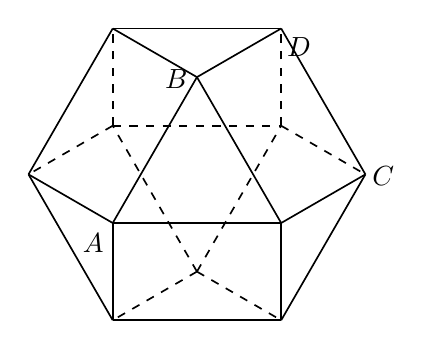
\begin{tikzpicture}[scale=0.95, semithick, every node/.style={inner sep=1.5pt}]
  % 可见棱
  \draw (-1.126,-1.950) -- (-2.252,0.000);
  \draw (-1.126,-1.950) -- (1.126,-1.950);
  \draw (-1.126,-1.950) -- (-1.126,-0.650);
  \draw (-2.252,0.000) -- (-1.126,1.950);
  \draw (-2.252,0.000) -- (-1.126,-0.650);
  \draw (1.126,-1.950) -- (2.252,0.000);
  \draw (1.126,-1.950) -- (1.126,-0.650);
  \draw (-1.126,1.950) -- (1.126,1.950);
  \draw (-1.126,1.950) -- (0.000,1.300);
  \draw (-1.126,-0.650) -- (1.126,-0.650);
  \draw (-1.126,-0.650) -- (0.000,1.300);
  \draw (2.252,0.000) -- (1.126,1.950);
  \draw (2.252,0.000) -- (1.126,-0.650);
  \draw (1.126,1.950) -- (0.000,1.300);
  \draw (1.126,-0.650) -- (0.000,1.300);
  % 被遮挡棱
  \draw[dashed] (0.000,-1.300) -- (-1.126,0.650);
  \draw[dashed] (0.000,-1.300) -- (-1.126,-1.950);
  \draw[dashed] (0.000,-1.300) -- (1.126,0.650);
  \draw[dashed] (0.000,-1.300) -- (1.126,-1.950);
  \draw[dashed] (-1.126,0.650) -- (-2.252,0.000);
  \draw[dashed] (-1.126,0.650) -- (1.126,0.650);
  \draw[dashed] (-1.126,0.650) -- (-1.126,1.950);
  \draw[dashed] (1.126,0.650) -- (2.252,0.000);
  \draw[dashed] (1.126,0.650) -- (1.126,1.950);
  % 标注：A=(0,1,1)、B=(1,1,0)、C=(1,-1,0)、D=(1,0,-1) 四个顶点
  \node[below left]  at (-1.18,-0.72) {$A$};
  \node[left]        at (-0.06,1.28) {$B$};
  \node[right]       at (2.28,-0.02) {$C$};
  \node[below right] at (1.14,1.90) {$D$};
\end{tikzpicture}
\end{center}
\nopagebreak[4]
\end{question}
\begin{question}
\gkti{14}为求解方程 $x^5-1=0$ 的虚根，可以把原方程变形为 $(x-1)(x^4+x^3+x^2+x+1)=0$，再变形为 $(x-1)(x^2+ax+1)(x^2+bx+1)=0$，由此可得原方程的一个虚根为\gkblank{}。

\end{question}
\gkpart{二、选择题（本大题满分 20 分）}

本大题共有 4 题，每题有且只有一个正确答案，考生应在答题纸的相应编号上，将代表答案的小方格涂黑，选对得 5 分，否则一律得零分。

\begin{question}
\gkti{15}若向量 $\overrightarrow a=(2,0)$，$\overrightarrow b=(1,1)$，则下列结论正确的是\mbox{（　　）}

（A）$\overrightarrow a\cdot\overrightarrow b=1$

（B）$|\overrightarrow a|=|\overrightarrow b|$

（C）$(\overrightarrow a-\overrightarrow b)\perp\overrightarrow b$

（D）$\overrightarrow a\parallel\overrightarrow b$

\end{question}
\begin{question}
\gkti{16}函数 $f(x)=\dfrac{4^x-1}{2^x}$ 的图象关于\mbox{（　　）}

（A）原点对称

（B）直线 $y=x$ 对称

（C）直线 $y=-x$ 对称

（D）$y$ 轴对称

\end{question}
\begin{question}
\gkti{17}直线 $l:y=k\left(x+\dfrac12\right)$ 与圆 $C:x^2+y^2=1$ 的位置关系为\mbox{（　　）}

（A）相交或相切

（B）相交或相离

（C）相切

（D）相交

\end{question}
\begin{question}
\gkti{18}若 $\overrightarrow{a_1}$，$\overrightarrow{a_2}$，$\overrightarrow{a_3}$ 均为单位向量，则 $\overrightarrow{a_1}=\left(\dfrac{\sqrt3}3,\dfrac{\sqrt6}3\right)$ 是 $\overrightarrow{a_1}+\overrightarrow{a_2}+\overrightarrow{a_3}=(\sqrt3,\sqrt6)$ 的\mbox{（　　）}

（A）充分不必要条件

（B）必要不充分条件

（C）充分必要条件

（D）既不充分又不必要条件

\end{question}
\gkpart{三、解答题（本大题满分 74 分）}

本大题共有 5 题，解答下列各题必须在答题纸相应编号的规定区域内写出必要的步骤。

\begin{question}
\gkti{19}\textbf{（本题满分 12 分）} 已知向量 $\overrightarrow a=(\sin2x-1,\cos x)$，$\overrightarrow b=(1,2\cos x)$。设函数 $f(x)=\overrightarrow a\cdot\overrightarrow b$，求函数 $f(x)$ 的最小正周期及 $x\in\left[0,\dfrac\pi2\right]$ 时的最大值。

\Needspace{0.4\textheight}
\end{question}
\begin{question}
\gkti{20}\textbf{（本题满分 14 分）} 某甜品店制作一种蛋筒冰淇淋，其上半部分呈半球形、下半部分呈圆锥形（如图）。现把半径为 $10\ \mathrm{cm}$ 的圆形蛋皮等分成 5 个扇形，用一个扇形蛋皮围成圆锥的侧面（蛋皮厚度忽略不计），求该蛋筒冰淇淋的表面积和体积（精确到 $0.01$）。
\nopagebreak[4]
\begin{center}% 2011 年上海春季卷第 20 题：蛋筒冰淇淋（上半为半球，下半为圆锥）
% 来源 PDF：春季高考/2011/2011春季上海.pdf，第 2 页（原刊 2-33 页）第 1 栏。
% 重绘依据：原图为正视图示意：上方半球与下方倒立圆锥在开口处相接，开口画成椭圆虚线。
\begin{tikzpicture}[scale=1.0, semithick]
  % 半球（上）
  \draw (-1.3,0) arc[start angle=180, end angle=0, radius=1.3];
  % 圆锥
  \draw (-1.3,0) -- (0,-2.6) -- (1.3,0);
  % 交接椭圆（虚线）
  \draw[dashed] (0,-0.28) ellipse[x radius=1.3, y radius=0.28];
  % 中心线与顶点
  \draw[dash dot] (0,1.55) -- (0,-2.8);
  \fill (0,-2.6) circle (1.6pt);
  \node[right] at (1.45,0.9) {半球};
  \node[right] at (1.05,-1.6) {圆锥};
\end{tikzpicture}
\end{center}
\nopagebreak[4]
\end{question}
\begin{question}
\gkti{21}\textbf{（本题满分 14 分）本题共有 2 个小题，第 1 小题满分 4 分，第 2 小题满分 10 分。} 

已知抛物线 $F:x^2=4y$。

（1） $\triangle ABC$ 的三个顶点在抛物线 $F$ 上，记 $\triangle ABC$ 的三边 $AB$，$BC$，$CA$ 所在直线的斜率分别为 $k_{AB}$，$k_{BC}$，$k_{CA}$，若点 $A$ 在坐标原点，求 $k_{AB}-k_{BC}+k_{CA}$ 的值；

（2） 请你给出一个以 $P(2,1)$ 为顶点、且其余各顶点均为抛物线 $F$ 上的动点的多边形，写出多边形各边所在直线的斜率之间的关系式，并说明理由。

说明：第（2）题将根据结论的一般性程度给予不同的评分。

\end{question}
\begin{question}
\gkti{22}\textbf{（本题满分 16 分）本题共有 3 个小题，第 1 小题满分 6 分，第 2 小题满分 6 分，第 3 小题满分 4 分。} 

定义域为 $\mathbf R$，且对任意实数 $x_1$，$x_2$ 都满足等式 $f\left(\dfrac{x_1+x_2}2\right)\leqslant\dfrac{f(x_1)+f(x_2)}2$ 的所有函数 $f(x)$ 组成的集合记为 $M$。例如，函数 $f(x)=kx+b\in M$。

（1） 已知函数 $f(x)=\begin{cases}x,&x\geqslant0,\\ \dfrac12x,&x<0.\end{cases}$ 证明：$f(x)\in M$；

（2） 写出一个函数 $f(x)$，使得 $f(x)\notin M$，并说明理由；

（3） 写出一个函数 $f(x)\in M$，使得数列极限 $\lim\limits_{n\to\infty}\dfrac{f(n)}{n^2}=1$，$\lim\limits_{n\to\infty}\dfrac{f(-n)}{-n}=1$。

\end{question}
\begin{question}
\gkti{23}\textbf{（本题满分 18 分）本题共有 3 个小题，第 1 小题满分 4 分，第 2 小题满分 8 分，第 3 小题满分 6 分。} 

\Needspace{5\baselineskip}
对于给定首项 $x_0>\sqrt[3]a$（$a>0$），由递推式
\nopagebreak[4]
\[x_{n+1}=\frac12\left(x_n+\sqrt{\frac a{x_n}}\right)\quad(n\in\mathbf N)\]
得到数列 $\{x_n\}$，且对于任意的 $n\in\mathbf N$，都有 $x_n>\sqrt[3]a$。用数列 $\{x_n\}$ 可以计算 $\sqrt[3]a$ 的近似值。

（1） 取 $x_0=5$，$a=100$，计算 $x_1$，$x_2$，$x_3$ 的值（精确到 $0.01$）；归纳出 $x_n$，$x_{n+1}$ 的大小关系；

（2） 当 $n\geqslant1$ 时，证明：$x_n-x_{n+1}<\dfrac12(x_{n-1}-x_n)$；

（3） 当 $x_0\in[5,10]$ 时，用数列 $\{x_n\}$ 计算 $\sqrt[3]{100}$ 的近似值，要求 $|x_n-x_{n+1}|<10^{-4}$，请你估计 $n$，并说明理由。

\clearpage

\end{question}